
\documentclass[journal,12pt,twocolumn]{IEEEtran}
\usepackage{graphicx}
\usepackage{listings}
\usepackage[utf8]{inputenc}
\usepackage{caption}
\usepackage{hyperref}
\usepackage[cmex10]{amsmath}
\usepackage{array}
\usepackage{gensymb}
\usepackage{booktabs}
\usepackage{etoolbox}
\patchcmd{\section}{\centering}{}{}{}
\providecommand{\norm}[1]{\left\lVert#1\right\rVert}
\providecommand{\abs}[1]{\left\vert#1\right\vert}
\let\vec\mathbf
\newcommand{\myvec}[1]{\ensuremath{\begin{pmatrix}#1\end{pmatrix}}}
\newcommand{\mydet}[1]{\ensuremath{\begin{vmatrix}#1\end{vmatrix}}}
\providecommand{\brak}[1]{\ensuremath{\left(#1\right)}}
\providecommand{\lbrak}[1]{\ensuremath{\left(#1\right.}}
\providecommand{\rbrak}[1]{\ensuremath{\left.#1\right)}}
\providecommand{\sbrak}[1]{\ensuremath{{}\left[#1\right]}}
\makeatletter
\newcommand\xleftrightarrow[2][]{%
  \ext@arrow 9999{\longleftrightarrowfill@}{#1}{#2}}
\newcommand\longleftrightarrowfill@{%
  \arrowfill@\leftarrow\relbar\rightarrow}
\makeatother
\title{Matrix Problems \textbf{\\Circles }}
\author{Manoj Chavva} 

\begin{document}
\maketitle



\section{Problem Statement}

\noindent The two circles $x^2+y^2=ax$ and $x^2+y^2=c^2 (c>0)$ touch each other if:
\begin{enumerate}
 
\item $2|a|=c $ 
\item $|a|=c$
\item $a=2c$
\item $|a| =2c$
\end{enumerate}

\section{Construction}
\begin{figure}[h] 
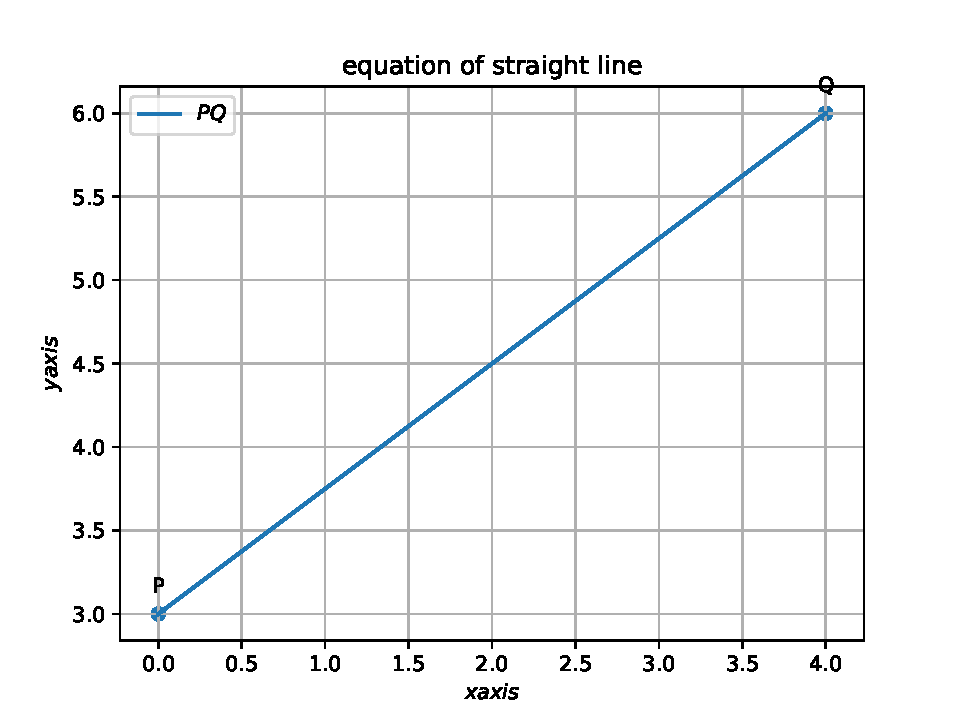
\includegraphics[width=1\columnwidth]{figure.pdf}
\caption{Figure of construction}
\label{fig:triangle}
\end{figure}


\section{Solution}
\noindent Circle equation 1 : $x^2+y^2=ax$\\
Circle equation 2 : $x^2+y^2=c^2 $ \\
The standard equation of the conics is given as :
\begin{align}
\vec{x}^{\top}\vec{V}\vec{x}+2\vec{u}^{\top}\vec{x}+f=0
\end{align}
The given circle 1 can be expressed as conics with \\parameters
	\begin{align}
	\vec{V_1} &= \vec{I}, \vec{u_1} = \myvec{\frac{a}{2} \\0}, f_1 = 0
	\end{align}
	Radius and Centre are
	\begin{align}
	r_1 &=\sqrt{{\vec{u}^{\top}\vec{u}}-f },
	\vec{a}=-u
    \end{align}
    \begin{align}
	r_1 = \sqrt{\frac{a}{2}*\frac{a}{2}}, \\
	r_1  = \pm \frac{a}{2}	
    \end{align}
    
\noindent The given circle 2 can be expressed as conics with \\parameters
    \begin{align}
	\vec{V_2} &= \vec{I}, \vec{u_2} = \myvec{0 \\0}, f_2 = -c^2
	\end{align}
	Radius and Centre are
	\begin{align}
	r_2 &=\sqrt{{\vec{u}^{\top}\vec{u}}-f }
    \end{align}
    \begin{align}
	r_2 &=\sqrt{{0}-(-c^2) }
    \end{align}
    \begin{align}
	r_2 &=\pm c 
    \end{align}


\begin{table}[h]
\centering
\large
\begin{tabular}{|l|l|l|}
\hline
\textbf{Symbol} & \textbf{Value} & \textbf{Description} \\ \hline
a               & 6         &  Input Circle Radius             \\ \hline
$\vec{u_1}$              & $\myvec{\frac{a}{2} \\ 0}$         &  Centre of circle 1             \\ \hline
$\vec{u_2}$             & $\myvec{0\\0}$       & Centre of Circle2             \\ \hline

\end{tabular}
\end{table}

\noindent Distance between centres $u_1$ and $u_2 $ is given by
\begin{align}
\norm{\vec{u_1}-\vec{u_2}}= \pm \frac{a}{2}
\end{align}
 \noindent The two circles will touch each other iff.
 \begin{align}
r_1 \pm r_2 = \norm{\vec{u_1}-\vec{u_2}}
\end{align}
\begin{align}
r_1 \pm r_2 = \pm \frac{a}{2}
\end{align}
\begin{align}
\pm \frac{a}{2} +c = \pm \frac{a}{2}
\end{align}
\begin{align}
c = |a|
\end{align}
Hence, option 2 is correct.
\begin{table}[h]
\large
\begin{tabular}{lll}
\multicolumn{3}{l}{Get Python Code for image from}                                                 \\ \hline
\multicolumn{3}{|l|}{\url{https://github.com/ManojChavva/FWC/blob/main/Matrix/circle/codes/circle.py}} \\ 
 \hline
\multicolumn{3}{l}{Get LaTex code from}                                                            \\ \hline
\multicolumn{3}{|l|}{\url{https://github.com/ManojChavva/FWC/blob/main/Matrix/circle/circle.tex}}            \\ \hline
\end{tabular}
\end{table}

\end{document}


